\documentclass[aspectratio=169]{beamer}

\usetheme{default}
\usecolortheme{default}
\setbeamertemplate{navigation symbols}{}
\setbeamertemplate{footline}[frame number]

\usepackage[T1]{fontenc}
\usepackage[utf8]{inputenc}
\usepackage{lmodern}
\usepackage{graphicx}
\usepackage{tikz}
\usepackage[backend=biber]{biblatex}

\addbibresource{references.bib}

\setbeamercolor{background canvas}{bg=white}
\setbeamercolor{normal text}{fg=black,bg=white}
\setbeamercolor{frametitle}{fg=black,bg=white}
\setbeamercolor{title}{fg=black,bg=white}

\newcommand{\figureplaceholder}[1]{%
  \begin{tikzpicture}
    \draw[black!45, line width=0.8pt] (0,0) rectangle (0.98\linewidth,0.52\textheight);
    \node[text=black!60] at (0.49\linewidth,0.26\textheight) {#1};
  \end{tikzpicture}
}

\title{Questions on Correlated Uncertainties}
\author{}
\date{November 23, 2026}

\newcommand{\figslide}[3]{\begin{frame}{#1}\centering\includegraphics[width=\textwidth,height=0.78\textheight,keepaspectratio]{#2}\par\vspace{0.05cm}{\footnotesize #3}\end{frame}}
\begin{document}

\begin{frame}
  \titlepage
\end{frame}

\begin{frame}{Main Questions}
  \begin{itemize}
    \item Quantify the effect of including correlated experimental uncertainties in the likelihood on the posterior distribution.
    \item Search for inference methods capable of estimating correlated experimental uncertainties from data.
  \end{itemize}
\end{frame}

\begin{frame}
  \centering
  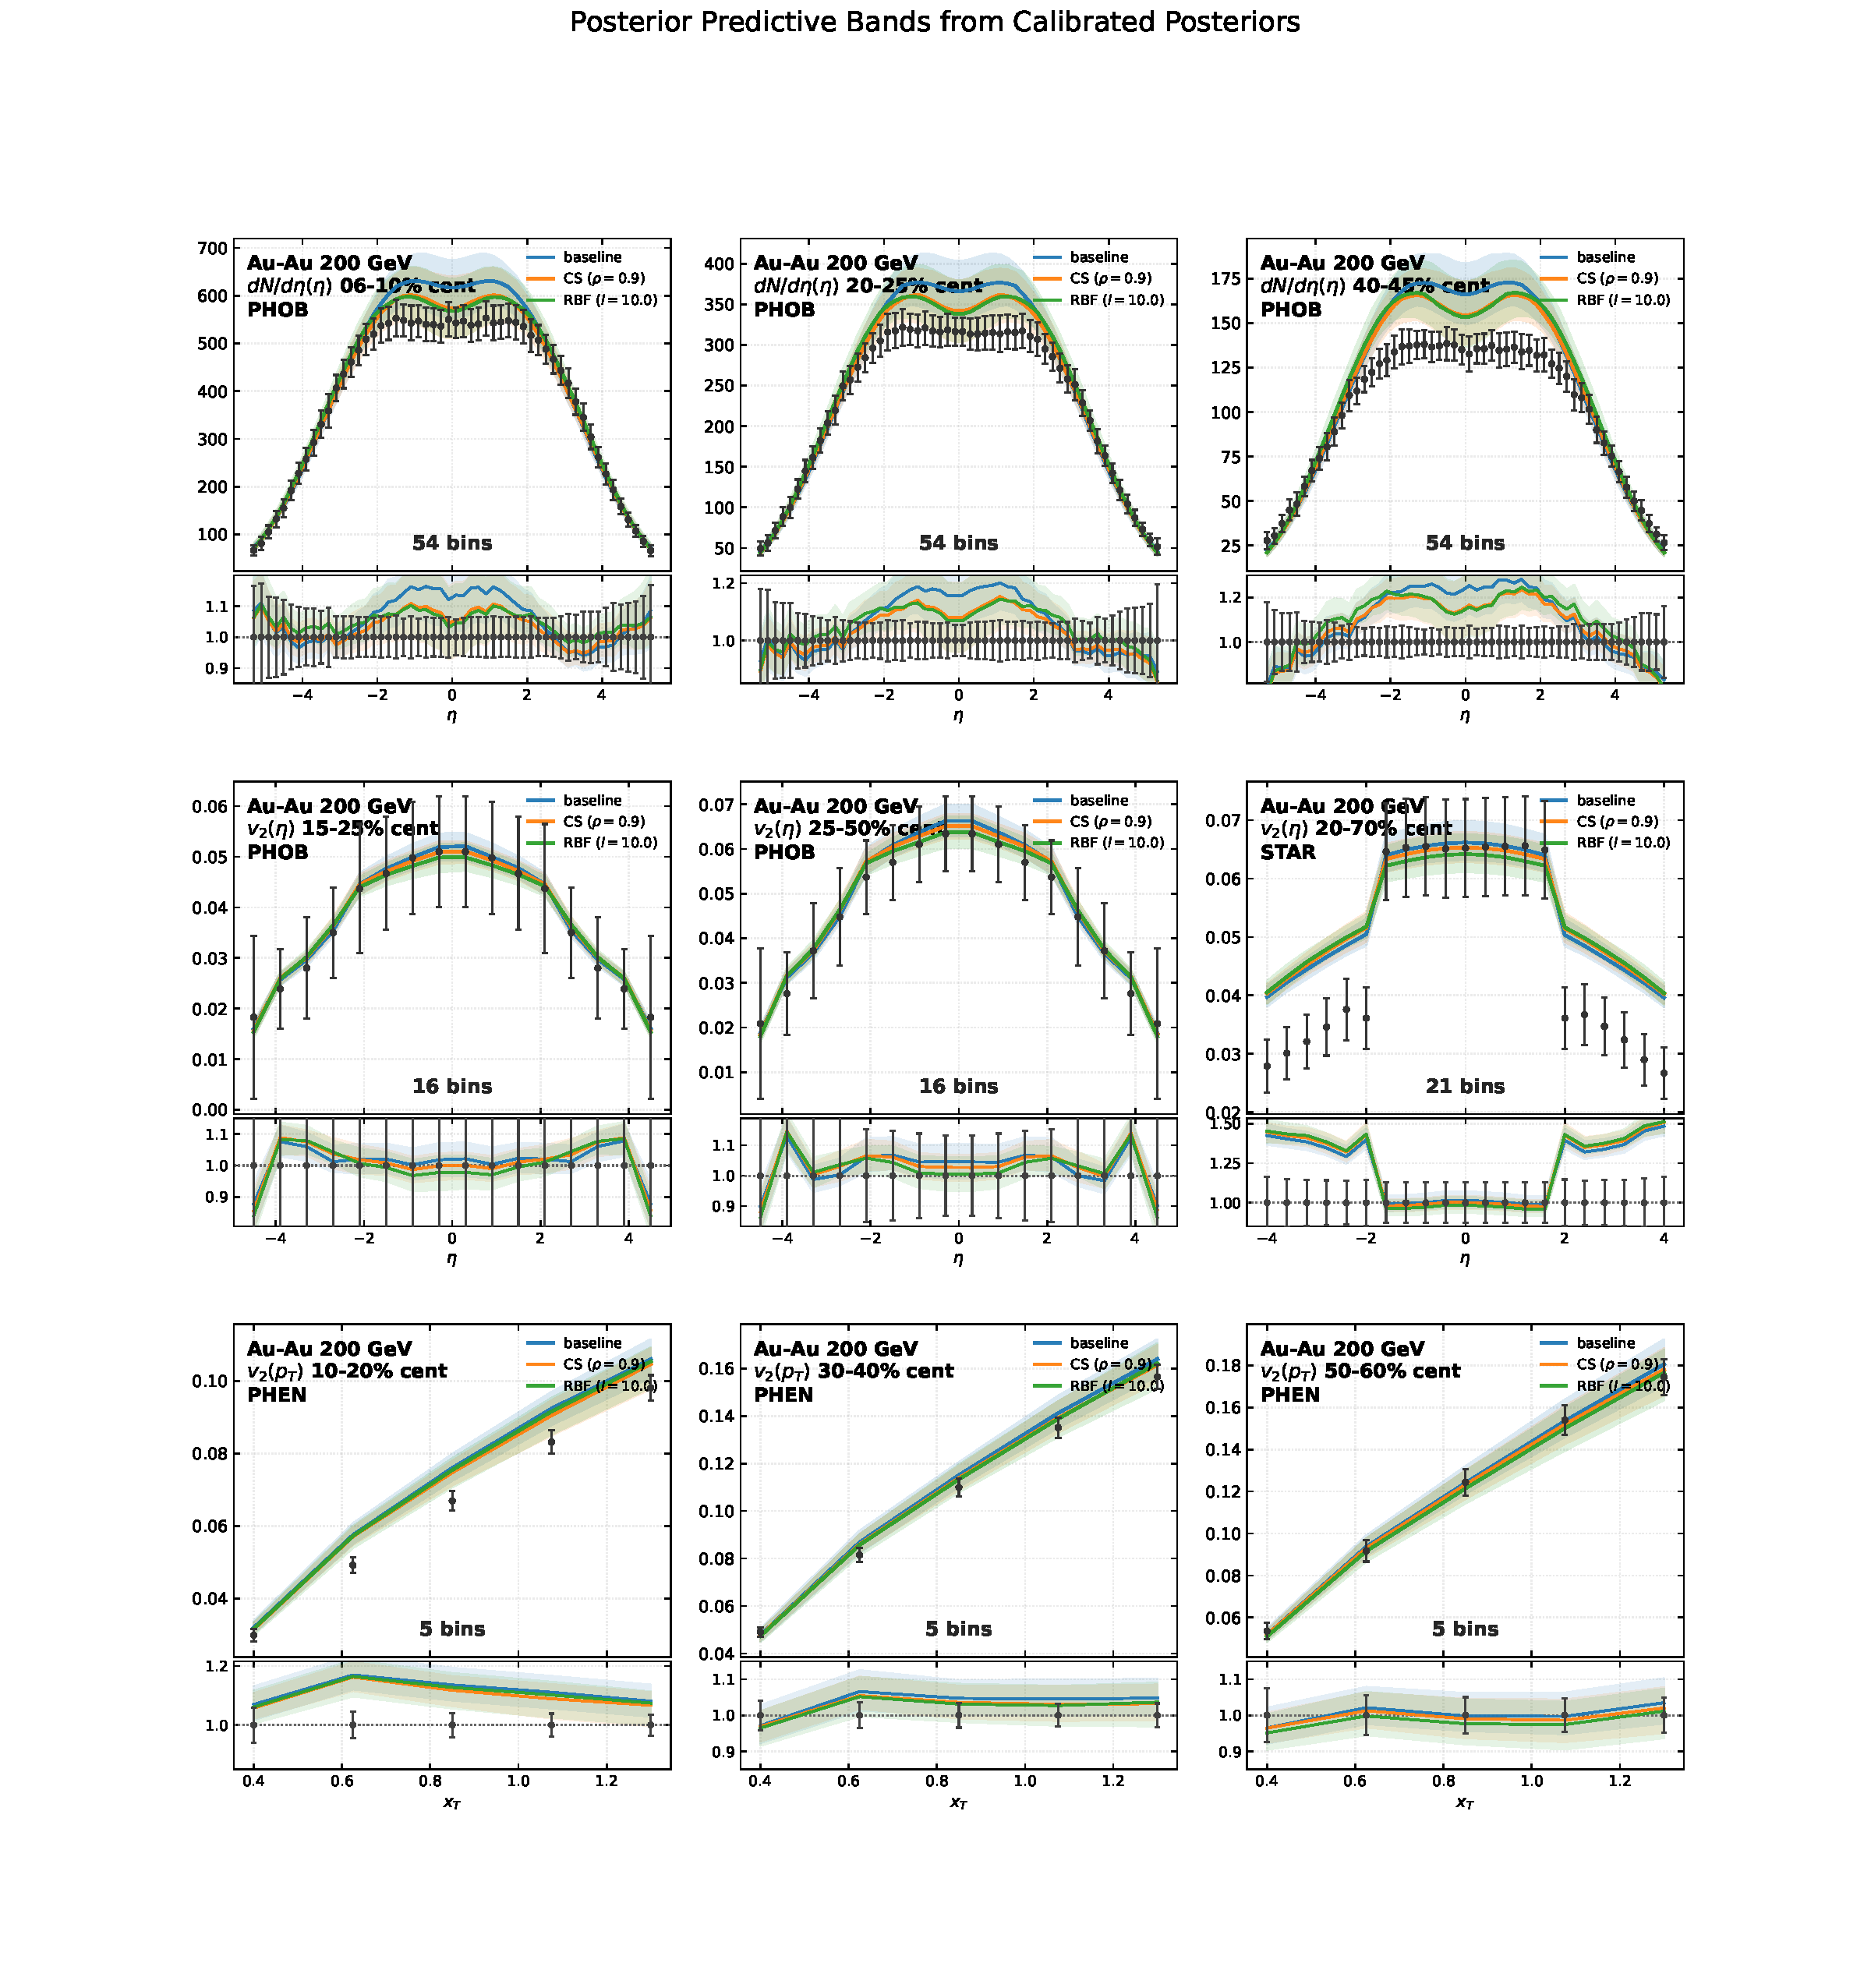
\includegraphics[width=1.06\textwidth,height=0.90\textheight,keepaspectratio]{img/posterior.pdf}
  \vspace{0.05cm}

  {\footnotesize Posterior distributions obtained with and without correlated uncertainty information in the likelihood.}
\end{frame}


\begin{frame}{Outline}\tableofcontents\end{frame}

\section{Sensitivity test: global}
\figslide{Global: baseline vs CS vs RBF}{img/1-First_sensitivity_test_global/long_global_baseline_cs_rbf_posterior_marginals.png}{Marginal posteriors of the 20 parameters: baseline (diagonal, blue), CS global $\rho=1$ (red), RBF global $\ell=0.5$ (orange). 200 walkers, 20k burn-in + 20k production.}
\figslide{Global: baseline vs CS}{img/1-First_sensitivity_test_global/long_global_cs_posterior_marginals_comparison.png}{Fully correlated (CS) experimental errors barely move the posteriors; largest shift: $\alpha_{\mathrm{shadowing}}$ ($-0.5\sigma$).}
\figslide{Global: baseline vs RBF}{img/1-First_sensitivity_test_global/long_global_rbf_posterior_marginals_comparison.png}{Global RBF correlation: small shifts, mainly in $\zeta/s$ parameters ($\lesssim 0.4\sigma$).}
\figslide{Global: joint posteriors}{img/1-First_sensitivity_test_global/long_global_baseline_cs_rbf_posterior_corner.pdf}{All 2D posteriors (68\% and 90\% contours) for the three error models.}
\figslide{Global: shift vs exp/emulator variance}{img/1-First_sensitivity_test_global/long_global_shift_vs_cov_ratio.png}{Posterior mean shift vs ratio $\sigma^2_{\mathrm{exp}}/\sigma^2_{\mathrm{emu}}$ seen by each parameter: weak correlation (Spearman 0.25 CS, 0.39 RBF).}
\figslide{Global: posterior predictive}{img/1-First_sensitivity_test_global/posterior_predictive/posterior_predictive_selected_9panels_legends_all_axes.png}{Model predictions from each posterior vs data: CS pushes $dN/d\eta$ up at mid-rapidity; $v_2$ almost unchanged.}

\section{Sensitivity test: sector}
\figslide{Sector: baseline vs CS}{img/2-Second_sensitivity_test_sector/sector_cs_posterior_marginals_comparison.png}{Correlations only inside rapidity sectors (CS, $\rho=1$) vs diagonal baseline.}
\figslide{Sector: baseline vs RBF}{img/2-Second_sensitivity_test_sector/sector_rbf_posterior_marginals_comparison.png}{Correlations only inside rapidity sectors (RBF) vs diagonal baseline.}
\figslide{Sector: joint posteriors (CS)}{img/2-Second_sensitivity_test_sector/sector_cs_vs_baseline_posterior_corner.png}{2D posteriors, CS sector vs baseline.}
\figslide{Sector: joint posteriors (RBF)}{img/2-Second_sensitivity_test_sector/sector_rbf_vs_baseline_posterior_corner.png}{2D posteriors, RBF sector vs baseline.}
\figslide{Sector and global: shift vs variance ratio}{img/2-Second_sensitivity_test_sector/sector_shift_vs_cov_ratio.png}{Median shift vs emulator/experimental variance ratio ($x$ axis here is $\sigma^2_{\mathrm{emu}}/\sigma^2_{\mathrm{exp}}$).}

\section{Sensitivity test: asymmetrical distribution (gamma)}
\figslide{Non-Gaussian noise: STAR $v_2(\eta)$}{img/3-Third_sensitivity_test_third_cov_momentum/a_global_nuisance/star_v2_eta_corrected_3way.png}{STAR $v_2(\eta)$ 20--70\%: skewed (gamma) nuisance terms for normalization, asymmetry and edges.}
\figslide{Non-Gaussian noise: nuisance posteriors}{img/3-Third_sensitivity_test_third_cov_momentum/a_global_nuisance/nuisance_lambda_prior_posterior.png}{Prior vs posterior of the nuisance amplitudes $\lambda$.}
\figslide{Non-Gaussian noise: parameter posteriors}{img/3-Third_sensitivity_test_third_cov_momentum/a_global_nuisance/posterior_marginals_3way.png}{Baseline vs CS sector vs non-Gaussian nuisance.}
\figslide{Detector split (TPC / FTPC)}{img/3-Third_sensitivity_test_third_cov_momentum/b_detector_split/posterior_marginals_4way.png}{Separate normalization for TPC and FTPC: four-way comparison.}
\figslide{Detector split: shifts}{img/3-Third_sensitivity_test_third_cov_momentum/b_detector_split/shift_summary.png}{Posterior shifts for each error model.}
\figslide{Detector split: STAR $v_2(\eta)$}{img/3-Third_sensitivity_test_third_cov_momentum/b_detector_split/star_v2_eta_corrected_4way.png}{Corrected STAR $v_2(\eta)$ with the detector-split nuisance.}
\figslide{Recovering the noise sources}{img/3-Third_sensitivity_test_third_cov_momentum/a_global_nuisance/sources_true_vs_recovered.png}{True vs recovered non-Gaussian sources.}

\section{GP heuristics}
\begin{frame}{GP fit of correlated uncertainty}
  \centering
  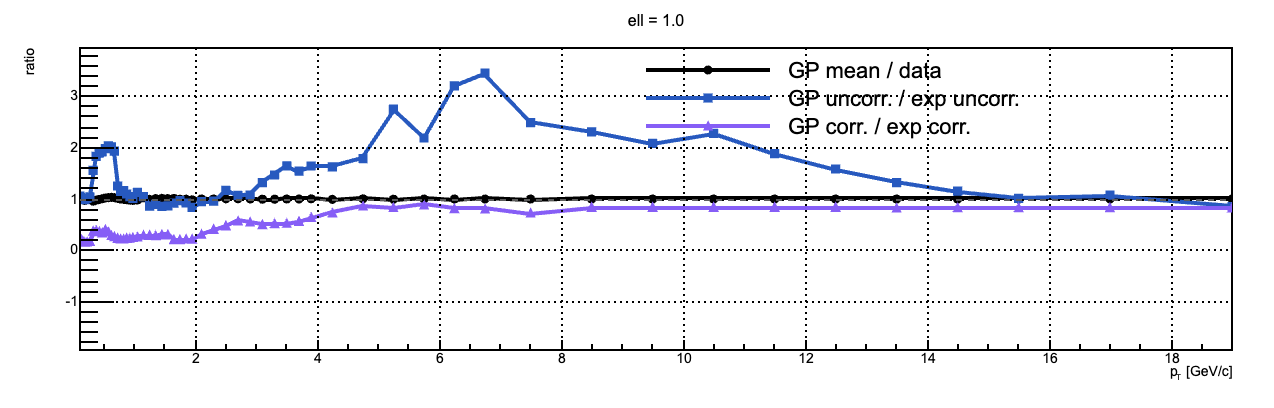
\includegraphics[width=1.06\textwidth,height=0.80\textheight,keepaspectratio]{img/Atlas-ell-1.0.png}
  \vspace{0.05cm}

  {\footnotesize Experimental correlated uncertainty fit through Gaussian Process.}
\end{frame}

\begin{frame}{Next Steps}
  \begin{itemize}
    \item Study methods for inferring uncertainty correlations from experimental data.
    \item Repeat the analysis of DOI:10.1103/7kjw-vfgp using the inferred correlation structure.
  \end{itemize}
\end{frame}

\end{document}
